\documentclass[border=2pt]{standalone}
\usepackage{amsmath, amsthm, amsfonts}
\usepackage{tikz-cd, kotex}
\usepackage{quiver}
\usepackage{Operators}
\usepackage{palette}
\usepackage{diagram-style}
\usetikzlibrary{arrows.meta, positioning}
\begin{document}

%%FIG Hasse diagram of Bruhat order for Gr(2,4) (Bruhat_Decomposition-1.svg)
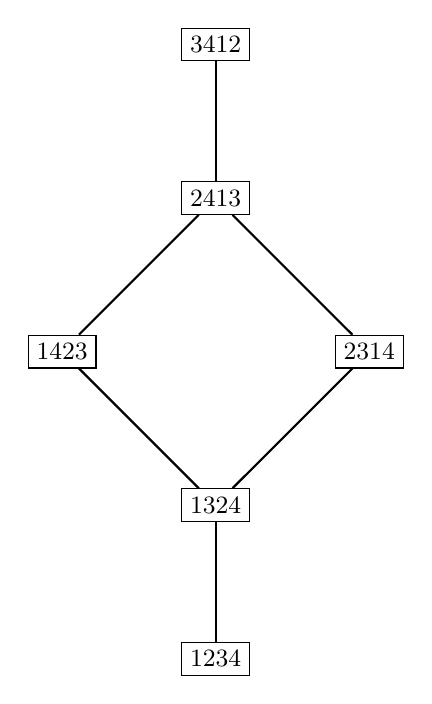
\begin{tikzpicture}[scale=1.3, node/.style={draw, fill=white, inner sep=3pt, font=\small}, edge/.style={thick}]
  \node[node] (n0) at (0,0) {$1234$};
  \node[node] (n1) at (0,1.5) {$1324$};
  \node[node] (n2a) at (-1.5,3) {$1423$};
  \node[node] (n2b) at (1.5,3) {$2314$};
  \node[node] (n3) at (0,4.5) {$2413$};
  \node[node] (n4) at (0,6) {$3412$};
  \draw[edge] (n0)--(n1);
  \draw[edge] (n1)--(n2a);
  \draw[edge] (n1)--(n2b);
  \draw[edge] (n2a)--(n3);
  \draw[edge] (n2b)--(n3);
  \draw[edge] (n3)--(n4);
\end{tikzpicture}

\end{document}
